\chapter{初段ミューオントリガーシステム}
\section{ATLASトリガーシステム}

\section{ミューオン検出器}
\subsection{Thin Gap Chamber (TGC)}

\subsection{Resitive Plate Chamber (RPC)}

\subsection{New Small Wheel (NSW)}

\subsection{small-strip TGC (sTGC)}

\subsection{Micromegas (MM)}

\section{初段ミューオントリガー}

\subsection{トリガー領域の分割}
ROIの話
\subsection{初段ミューオントリガーにおけるミューオンの運動量の算出}
CWの話
\subsection{現行のトリガー性能}
現行の話

\section{本研究の目的}
\subsection{Run-2におけるCWの作成及び最適化手法}
\subsection{本研究の方針}


\begin{figure}[tb]
  \centering
  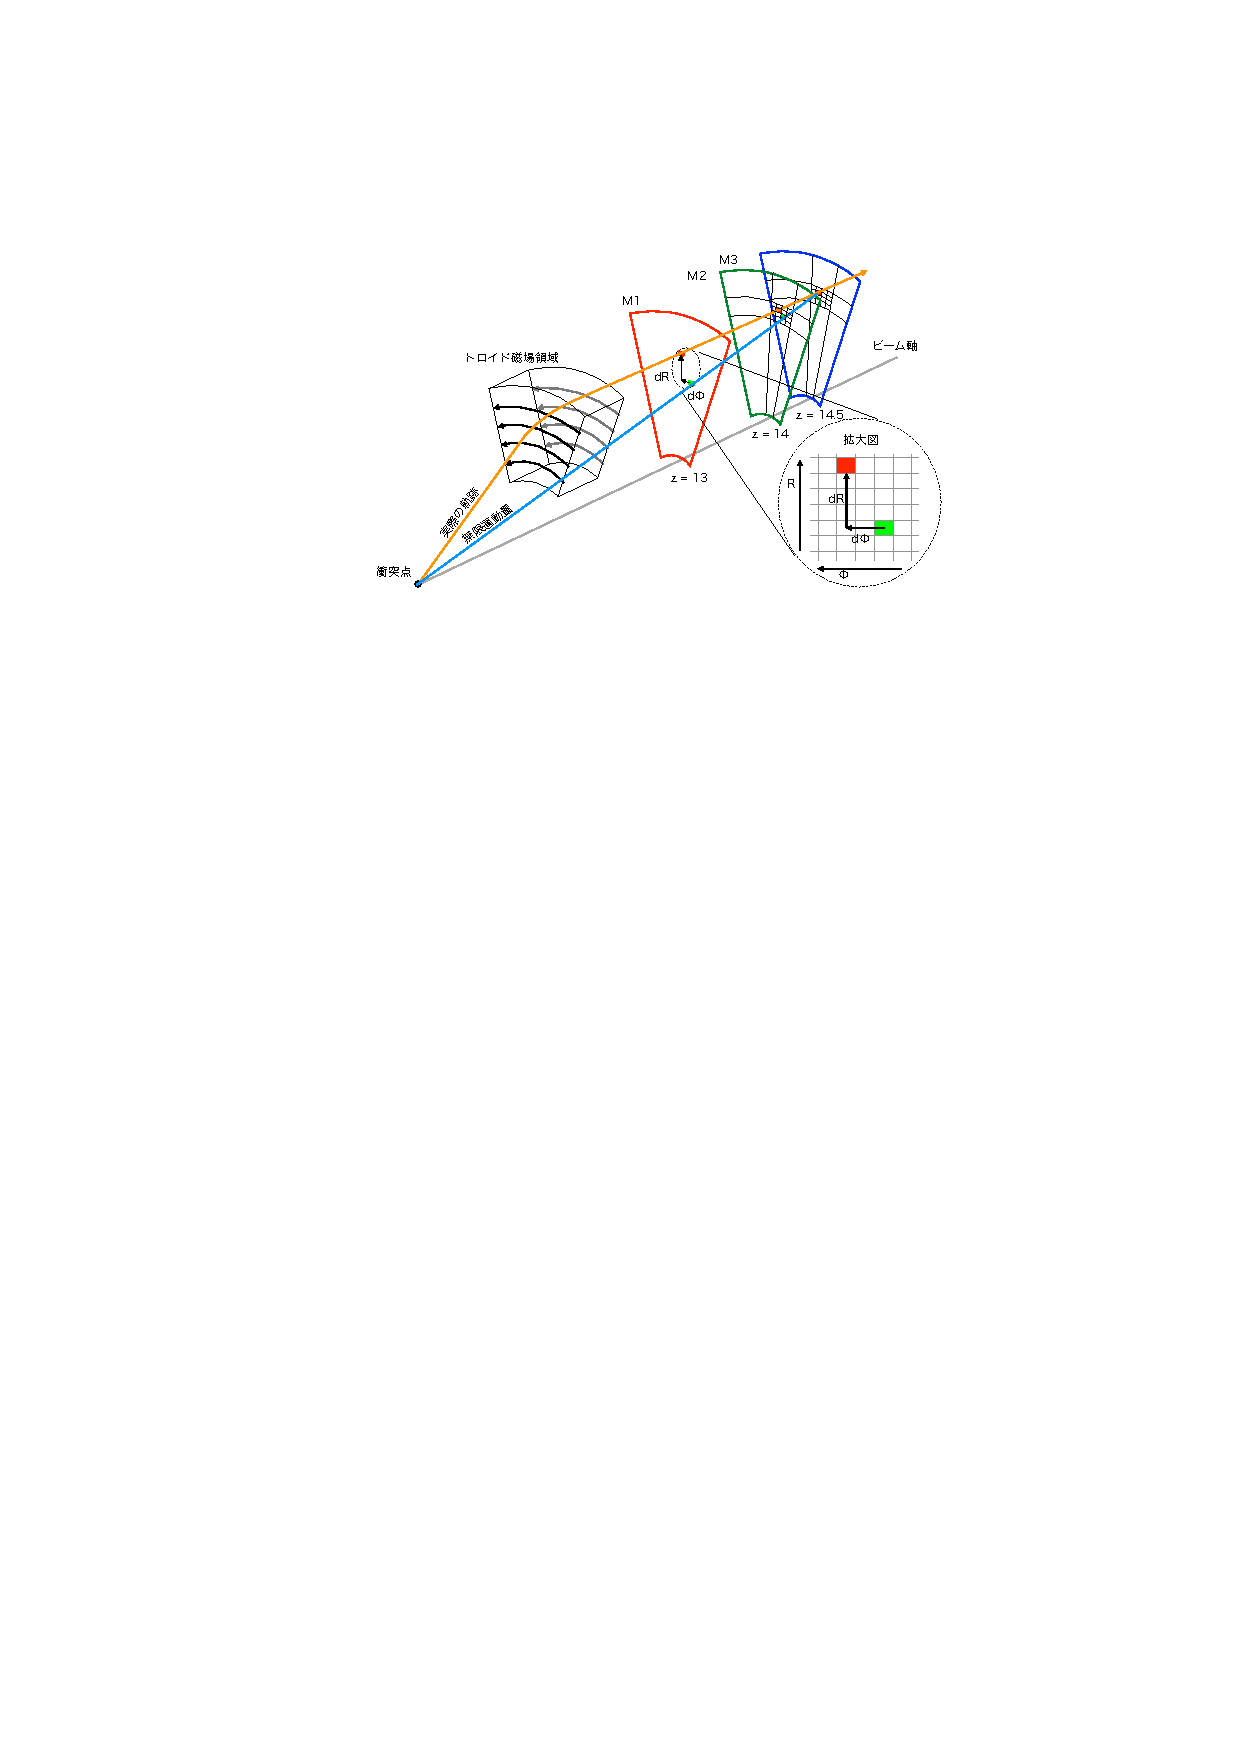
\includegraphics[clip, width=14cm]{fig/3/akatsuka_mt_trigger_scheme.pdf}
  \caption{ATLAS検出器エンドキャップ領域におけるトリガースキームの概念図\cite{article:akatsuka-mron}。無限大の運動量を持つミューオンを仮定し、磁場によって曲げられたミューオンとの位置の差を用いて$\pt$を計算する。}
  \label{fig:trigger-scheme}
\end{figure}









